% !TeX program = xelatex
% !TEX TS-program = xelatex
\documentclass[10pt]{article}
% Common packages for the Chinese experiment report.
% Compile with XeLaTeX.
\usepackage{fontspec}
\usepackage{xeCJK}
\usepackage{microtype}
\usepackage[letterpaper,margin=1in]{geometry}
\usepackage{graphicx}
\usepackage{amsmath,amssymb,mathbbol}
\usepackage{acronym}
\usepackage{enumitem}
\usepackage[pagebackref=true,breaklinks=true,colorlinks]{hyperref}
\usepackage{balance}
\usepackage{xspace}
\usepackage{setspace}
\usepackage{indentfirst}
\usepackage[skip=3pt,font=small]{subcaption}
\usepackage[skip=3pt,font=small]{caption}
\usepackage[dvipsnames]{xcolor}
\usepackage[capitalise]{cleveref}
\usepackage{booktabs,tabularx,colortbl,multirow,array,makecell}
\usepackage{siunitx}
\usepackage{float}

\IfFontExistsTF{Times New Roman}{\setmainfont{Times New Roman}}{\setmainfont{TeX Gyre Termes}}
\IfFontExistsTF{Helvetica}{\setsansfont{Helvetica}}{\setsansfont{TeX Gyre Heros}}
\IfFontExistsTF{Menlo}{\setmonofont{Menlo}}{\setmonofont{Inconsolata}}
\IfFontExistsTF{Songti SC}{
  \setCJKmainfont{Songti SC}[AutoFakeBold=2]
  \setCJKsansfont{Songti SC}[AutoFakeBold=2]
  \setCJKmonofont{Songti SC}[AutoFakeBold=2]
}{
  \setCJKmainfont{FandolSong-Regular.otf}[AutoFakeBold=2]
  \setCJKsansfont{FandolHei-Regular.otf}
  \setCJKmonofont{FandolSong-Regular.otf}
}

\hypersetup{pdfencoding=auto,colorlinks=true,allcolors=black}
\pagestyle{plain}

% Chinese document names.
\renewcommand{\figurename}{图}
\renewcommand{\tablename}{表}
\renewcommand{\refname}{参考资料}
\renewenvironment{abstract}%
{%
  \vskip 0.075in%
  \centerline%
  {\large\bf 摘要}%
  \vspace{0.5ex}%
  \begin{quote}%
  \setlength{\parindent}{2em}%
  \leavevmode\hspace*{2em}\ignorespaces%
}
{
  \par%
  \end{quote}%
  \vskip 1ex%
}

% Handy shorthand
\makeatletter
\DeclareRobustCommand\onedot{\futurelet\@let@token\@onedot}
\def\@onedot{\ifx\@let@token.\else.\null\fi\xspace}
\def\eg{\emph{e.g}\onedot}
\def\Eg{\emph{E.g}\onedot}
\def\ie{\emph{i.e}\onedot}
\def\Ie{\emph{I.e}\onedot}
\def\cf{\emph{c.f}\onedot}
\def\Cf{\emph{C.f}\onedot}
\def\etc{\emph{etc}\onedot}
\def\vs{\emph{vs}\onedot}
\def\wrt{w.r.t\onedot}
\def\dof{d.o.f\onedot}
\def\etal{\emph{et al}\onedot}
\makeatother

\definecolor{gray}{gray}{0.9}
\definecolor{reportgreen}{HTML}{008E7D}
\definecolor{reportorange}{HTML}{D97706}
\definecolor{reportslate}{HTML}{334155}

% Table style
\sisetup{
  detect-all,
  table-number-alignment = center,
  group-minimum-digits = 4
}
\newcolumntype{Y}{>{\raggedright\arraybackslash}X}
\newcolumntype{L}[1]{>{\raggedright\arraybackslash}p{#1}}
\renewcommand{\arraystretch}{1.12}

% Handy math ops
\DeclareMathOperator*{\argmax}{arg\,max}
\DeclareMathOperator*{\argmin}{arg\,min}
\newcommand{\norm}[1]{\left\Vert #1 \right\Vert}

% Spacing
\frenchspacing
\setstretch{1}
\setlength{\parindent}{2em}
\setlength{\parskip}{5.5pt}
\makeatletter
\renewcommand{\normalsize}{%
  \@setfontsize\normalsize\@xpt{13.75pt}%
  \abovedisplayskip      7\p@ \@plus 2\p@ \@minus 5\p@
  \abovedisplayshortskip \z@ \@plus 3\p@
  \belowdisplayskip      \abovedisplayskip
  \belowdisplayshortskip 4\p@ \@plus 3\p@ \@minus 3\p@
}
\normalsize
\makeatother
\setlength\floatsep{0.5\baselineskip plus 3pt minus 2pt}
\setlength\textfloatsep{0.5\baselineskip plus 3pt minus 2pt}
\setlength\dbltextfloatsep{0.5\baselineskip plus 3pt minus 2pt}
\setlength\intextsep{0.5\baselineskip plus 3pt minus 2pt}

\makeatletter
\renewcommand{\maketitle}{%
  \begin{center}
    {\LARGE\bfseries \@title\par}
    \vspace{1.2em}
    {\normalsize \@author\par}
  \end{center}
  \vspace{1.2em}
}
\makeatother

\makeatletter
\renewcommand{\paragraph}{%
  \@startsection{paragraph}{4}%
  {\z@}{0ex \@plus 0ex \@minus 0ex}{-1em}%
  {\hskip\parindent\normalfont\normalsize\bfseries}%
}
\makeatother

% Graphics path
\graphicspath{{figures/}}

% Clever references
\crefname{algorithm}{算法}{算法}
\Crefname{algorithm}{算法}{算法}
\crefname{section}{节}{节}
\Crefname{section}{节}{节}
\crefname{table}{表}{表}
\Crefname{table}{表}{表}
\crefname{figure}{图}{图}
\Crefname{figure}{图}{图}

% Acronym
\acrodef{ttft}[TTFT]{Time To First Token}
\acrodef{rss}[RSS]{Resident Set Size}


\title{本地 LLM Agent Prompt/KV 缓存复用的性能评估}
\author{%
  元培学院\quad 胡思成\quad2400017832\\
}
\date{}

\begin{document}
\maketitle

\begin{abstract}
\noindent 本地 Agent 在长上下文的多轮交互中通常会反复提交系统指令、工具定义、代码摘要或文档片段，而重复的 prefill 会显著推高首 token 延迟（time to first token, TTFT）。
为定量分析这一问题，本文测试了 \textbf{llama.cpp 本地服务中的 prompt/KV 缓存} 对 \textbf{coding agent 与 RAG agent} 的影响。
实验在 Apple M5、32 GB unified memory、Qwen2.5-Coder-3B-Instruct Q4\_K\_M 与单并发配置下运行，覆盖 2K、4K、8K、16K prompt 长度、三类缓存策略、动态字段位置敏感性以及 \texttt{--cache-reuse} 的参数扫描。
实验结果说明，\textbf{只在服务端打开缓存并不能保证 warm TTFT 改善}；如果动态字段位于 prompt 前部，缓存几乎无法发挥作用。
当稳定内容集中在 prompt 前缀中时，Coding 负载在 2K--16K 上获得 \textbf{17.0$\times$ 到 112.2$\times$} 的 TTFT 加速，RAG 负载获得 \textbf{13.6$\times$ 到 103.7$\times$} 的加速。
在 8K 布局实验中，\texttt{front\_volatile} 布局会把 warm TTFT 拉回 \textbf{9--12 秒量级}，而 \texttt{stable\_prefix}/\texttt{end\_volatile} 布局可以稳定在 \textbf{0.15--0.18 秒量级}。
当前单会话、稳定前缀设置下，\texttt{--cache-reuse} 的影响相对有限；绝大多数组合相对 reuse=0 的变化都在约 $\pm$10\% 以内。
因此，\textbf{本地 Agent 的 prompt 组织方式比单纯开启缓存更关键}，稳定、长且可复用的前缀应被视为系统级接口约束。
\end{abstract}

\section{引言}
\label{sec:introduction}

本地 LLM Agent 的一次请求往往不是单句问题，而是由多类上下文共同组成：代码摘要、相关文件、检索文档和历史摘要等内容会被拼接成一个长 prompt。
随着交互轮次增加，其中大量内容会跨轮保持不变，实际变化通常集中在当前用户问题、时间戳、request id、最新错误日志或少量对话状态。
如果服务端不能复用已经 prefill 的稳定前缀，这些重复上下文仍会在每一轮重新计算，首 token 延迟也会随 prompt 变长而快速上升。

因此，本文主要考察两个问题：prompt/KV 缓存能否把本地单机 Agent 服务中长上下文 warm turn 的 TTFT 降到接近短请求的水平；prompt 又应如何组织，才能稳定触发这种复用。
实验部分覆盖关闭缓存、默认缓存、稳定前缀、动态字段位置和 \texttt{--cache-reuse} 参数扫描等设置，用于区分“是否启用缓存”和“是否形成稳定可复用前缀”这两个因素。

\section{缓存复用机制}
\label{sec:theory}

对自回归 LLM 服务而言，一轮请求的首 token 延迟主要由三部分组成：新 token 的 prefill 计算、第一个 decode step，以及请求调度、序列化等固定开销。在输出长度固定或较短时，长上下文场景的差异主要来自 prefill。若上一轮已经保留了前缀的 KV 状态，warm turn 不必重新计算被命中的前缀；TTFT 可近似写为
\[
  T_{\mathrm{TTFT}} \approx T_{\mathrm{prefill}}(L_{\mathrm{new}}) + T_{\mathrm{decode},1} + T_{\mathrm{overhead}},
\]
其中 \(L_{\mathrm{new}} = L_{\mathrm{prompt}} - L_{\mathrm{reuse}}\) 表示未能复用、仍需重新 prefill 的 token 数。因此，缓存收益不只取决于是否启用缓存，更取决于跨轮 prompt 是否拥有足够长且完全一致的前缀。

后文将关闭缓存、默认缓存、稳定前缀和 \texttt{--cache-reuse} 参数扫描分别记为 S0--S3，具体服务端参数和 prompt 组织方式见表~\ref{tab:strategies}。

本文以 TTFT 作为核心指标，并同时记录总延迟、解码延迟、解码吞吐、输入 token 数、输出 token 数和服务端常驻内存集大小（resident set size, RSS）。这些指标由流式请求客户端与 \texttt{psutil} 采集。为了比较不同缓存配置的收益，加速比（speedup）统一定义为同一负载、同一 prompt 长度下的
\[
  \mathrm{speedup} = \frac{\mathrm{median\ TTFT}_{\mathrm{S0}}}{\mathrm{median\ TTFT}_{\mathrm{strategy}}}.
\]
因此，加速比大于 1 表示对应策略比关闭缓存更快。

在 S0 配置下，服务端关闭 prompt 缓存。即使 prompt 的大部分内容跨轮相同，每一轮也需要重新 prefill 完整上下文。理论上，warm TTFT 会随 prompt 长度近似单调增加；当 prompt 从 2K 扩展到 16K 时，prefill 成本应成为主要瓶颈。

在 S1 配置下，服务端虽然启用了缓存，但动态字段被放在 prompt 最前部。时间戳、request id 或当前用户请求只要在开头发生变化，后续原本稳定的系统指令、工具定义、代码片段或文档片段就不再构成可命中的公共前缀。此时有效的 \(L_{\mathrm{reuse}}\) 很小，理论表现应接近 S0；额外的缓存管理还可能带来少量开销。

在 S2 配置下，稳定内容被集中放在 prompt 前缀，动态字段集中后置。只要系统指令、工具定义、代码或文档上下文和长期摘要保持 token 序列一致，服务端就可以复用大部分 prefill 结果，warm turn 只需处理末尾新增或变化的短后缀。此时 \(L_{\mathrm{new}}\) 与总 prompt 长度弱相关，TTFT 应接近短请求水平，并且随着上下文变长获得更大的相对加速。

S3 在 S2 的稳定前缀基础上扫描 \texttt{--cache-reuse}。在单会话、单并发、前缀已经稳定的设置下，主要收益已经由 prompt 组织方式提供，reuse 参数只能影响剩余缓存状态的保留与匹配细节。理论上，它的边际影响应小于 S0/S1/S2 之间的结构性差异；只有在会话切换、上下文接近上限或复用边界频繁变化时，才可能成为主要因素。

\section{实验设置}
\label{sec:setup}

\subsection{硬件与软件环境}

\begin{table}[H]
  \caption{所有正式实验均在同一台本机上顺序运行，并固定为单并发，以减少 slot 调度和并发竞争带来的噪声。}
  \label{tab:environment}
  \centering
  \footnotesize
  \setlength{\tabcolsep}{5pt}
  \begin{tabularx}{0.85\linewidth}{@{}>{\bfseries}lY@{}}
    \toprule
    \textbf{项目} & \textbf{配置} \\
    \midrule
    机器 & MacBook Pro, Mac17,2 \\
    芯片与内存 & Apple M5，10-core CPU，10-core GPU，32 GB unified memory \\
    系统与架构 & macOS 26.4.1，Darwin arm64 \\
    推理服务 & \texttt{llama-server} version 9110，Metal enabled，OpenAI 兼容 API \\
    模型 & \texttt{qwen2.5-coder-3b-instruct-q4\_k\_m.gguf}，Qwen2.5-Coder-3B-Instruct，Q4\_K\_M \\
    Python 与依赖 & Python 3.11.14；\texttt{openai==2.36.0}，\texttt{psutil==7.2.2}，\texttt{pandas==3.0.3}，\texttt{numpy==2.4.4}，\texttt{matplotlib==3.10.9}，\texttt{seaborn==0.13.2} \\
    请求设置 & \texttt{temperature=0}，\texttt{top\_p=1}，\texttt{max\_tokens=64}，\texttt{--parallel 1} \\
    \bottomrule
  \end{tabularx}
\end{table}

\subsection{实验负载与缓存策略}

实验使用可控的合成负载，在固定任务语义的前提下改变缓存可复用前缀，避免任务内容差异干扰 TTFT 比较。Coding 负载模拟本地代码助手请求，prompt 由系统指令、工具定义、仓库结构、合成源文件、测试文件、对话摘要、动态元数据和当前用户请求组成。RAG 负载模拟长文档问答，prompt 由固定文档上下文和逐轮变化的问题组成。

每个请求序列包含 20 轮请求。统计时将第 1 轮作为 cold turn，正文主要报告第 2--20 轮 warm turn 的中位数。主实验策略见表~\ref{tab:strategies}。

\begin{table}[H]
  \caption{主实验缓存策略与 prompt 组织方式。}
  \label{tab:strategies}
  \centering
  \small
  \setlength{\tabcolsep}{5pt}
  \begin{tabularx}{\linewidth}{@{}>{\bfseries}lllY@{}}
    \toprule
    \textbf{编号} & \textbf{策略名} & \textbf{服务端参数} & \textbf{Prompt 组织方式} \\
    \midrule
    S0 & \texttt{no\_cache} & \texttt{--no-cache-prompt} & 使用 \texttt{stable\_prefix} 组织，但服务端关闭复用 \\
    S1 & \texttt{default\_cache} & \texttt{--cache-prompt} & 使用 \texttt{front\_volatile} 组织，动态字段位于 prompt 最前部 \\
    S2 & \textbf{\texttt{stable\_prefix}} & \texttt{--cache-prompt} & \textbf{系统指令、工具定义、代码或文档等稳定内容前置，动态字段后置} \\
    S3 & \begin{tabular}[t]{@{}l@{}}\texttt{cache-reuse}\\参数扫描\end{tabular} & \begin{tabular}[t]{@{}l@{}}\texttt{--cache-prompt}\\\texttt{--cache-reuse N}\end{tabular} & 沿用 S2 的组织方式，$N\in\{0,64,128,256,512\}$ \\
    \bottomrule
  \end{tabularx}
\end{table}

\section{实验结果}
\label{sec:results}

\subsection{缓存策略与 TTFT}
\label{sec:main-results}

图~\ref{fig:main-results} 的纵轴刻度间距按数值的对数排列，刻度标签仍为原始数值。

\begin{figure}[H]
  \centering
  \begin{subfigure}[t]{0.49\linewidth}
    \centering
    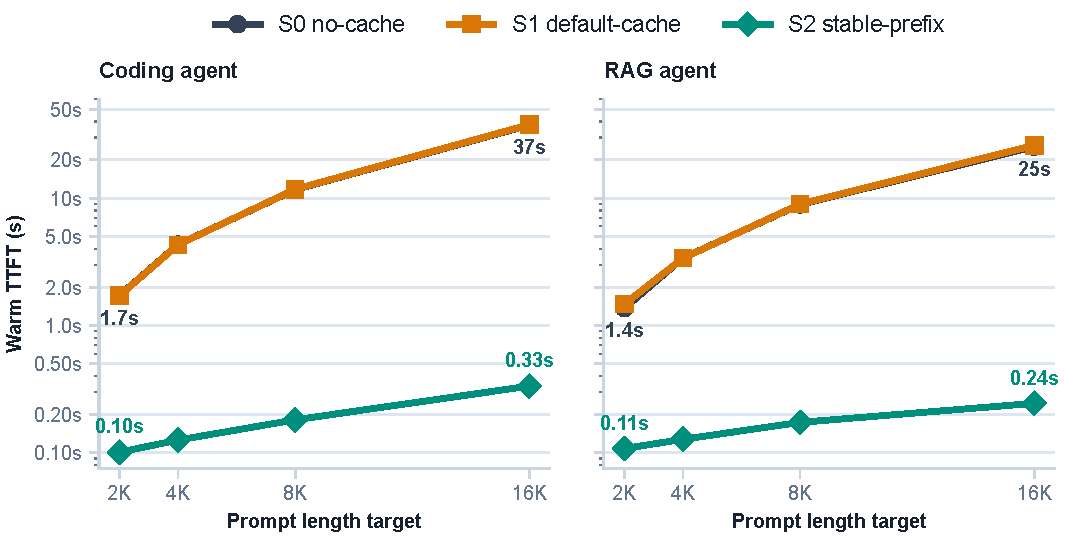
\includegraphics[width=\linewidth]{report_ttft_by_length}
    \caption{Warm TTFT}
    \label{fig:ttft-length}
  \end{subfigure}
  \hfill
  \begin{subfigure}[t]{0.49\linewidth}
    \centering
    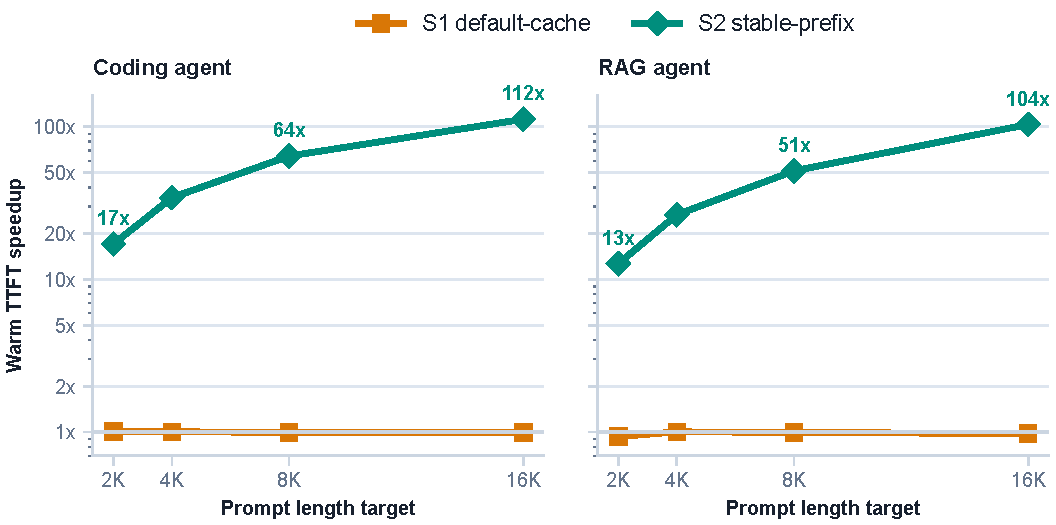
\includegraphics[width=\linewidth]{report_speedup_by_length}
    \caption{TTFT 加速比}
    \label{fig:speedup-length}
  \end{subfigure}
  \caption{主实验结果。}
  \label{fig:main-results}
\end{figure}

\begin{table}[H]
  \caption{\textbf{主实验 warm-turn 指标。}}
  \label{tab:main-results}
  \centering
  \footnotesize
  \setlength{\tabcolsep}{0pt}
  \begin{tabular*}{0.85\linewidth}{@{\extracolsep{\fill}}ll
    S[table-format=2.3]
    S[table-format=2.3]
    S[table-format=1.3,detect-weight=true]
    S[table-format=1.3]
    S[table-format=4.1]
    S[table-format=3.1,detect-weight=true]@{}}
    \toprule
    \multirow{2}{*}{\textbf{负载}} & \multirow{2}{*}{\textbf{长度}}
      & \multicolumn{3}{c}{\textbf{Warm TTFT (s) $\downarrow$}}
      & \multicolumn{2}{c}{\textbf{S2 指标}}
      & \multicolumn{1}{c}{\multirow{2}{*}{\textbf{speedup ($\times$) $\uparrow$}}} \\
    \cmidrule(lr){3-5}\cmidrule(lr){6-7}
      & & {\textbf{S0}} & {\textbf{S1}} & {\textbf{S2}}
      & {\textbf{总延迟 (s) $\downarrow$}}
      & {\textbf{RSS (MiB) $\downarrow$}}
      & \\
    \midrule
    \multirow{4}{*}{Coding}
      & 2K  & 1.724 & 1.715 & \bfseries 0.101 & 1.249 & 2277.0 & \bfseries 17.0 \\
      & 4K  & 4.319 & 4.302 & \bfseries 0.126 & 1.332 & 2432.2 & \bfseries 34.4 \\
      & 8K  & 11.661 & 11.728 & \bfseries 0.181 & 1.549 & 2742.5 & \bfseries 64.3 \\
      & 16K & 37.443 & 37.779 & \bfseries 0.334 & 2.268 & 3361.6 & \bfseries 112.2 \\
    \midrule
    \multirow{4}{*}{RAG}
      & 2K  & 1.369 & 1.468 & \bfseries 0.108 & 0.457 & 2274.9 & \bfseries 13.6 \\
      & 4K  & 3.386 & 3.378 & \bfseries 0.128 & 0.519 & 2427.8 & \bfseries 26.5 \\
      & 8K  & 8.908 & 8.952 & \bfseries 0.173 & 0.574 & 2732.7 & \bfseries 51.4 \\
      & 16K & 25.341 & 26.004 & \bfseries 0.244 & 0.630 & 3342.7 & \bfseries 103.7 \\
    \bottomrule
  \end{tabular*}
\end{table}

从主实验可以看出，关闭缓存时，TTFT 基本由长上下文 prefill 主导：Coding 负载从 2K 的 1.72 秒升至 16K 的 37.44 秒，RAG 负载从 1.37 秒升至 25.34 秒。这个增长不是简单的固定开销累加。以 Coding 为例，prompt 长度从 4K 到 8K 翻倍时，warm TTFT 从 4.32 秒升至 11.66 秒；从 8K 到 16K 再次翻倍时，进一步升至 37.44 秒。RAG 负载也呈现相同趋势，只是绝对值更低。这说明在当前本地后端和模型配置下，一旦不能复用前缀，长 prompt 的 prefill 会迅速成为首 token 延迟的主项，而不是一个可以被网络或 API 开销掩盖的小项。

S1 的结果提供了一个重要的反例：只把 \texttt{--cache-prompt} 打开，并不会自然得到 warm-cache 性能。S1 在 2K--16K 上的 TTFT 与 S0 基本重合，Coding 8K 甚至从 11.661 秒小幅变为 11.728 秒，RAG 16K 从 25.341 秒变为 26.004 秒。换言之，服务端确实被允许保留 prompt cache，但由于每轮开头的动态元数据不同，后续长段稳定内容无法成为同一个可命中的公共前缀。这一结果把“缓存开关”和“缓存命中条件”分开了：前者只是必要条件，后者才决定性能。

真正改变曲线的是 S2。S2 的 warm TTFT 随 prompt 长度增长很慢：Coding 从 2K 的 0.101 秒升至 16K 的 0.334 秒，RAG 从 0.108 秒升至 0.244 秒。虽然总 prompt 长度增加了 8 倍，S2 的绝对 TTFT 只增加到原来的约 3.3 倍和 2.3 倍；相比之下，S0 分别增加到约 21.7 倍和 18.5 倍。因此，S2 并不是把 prefill 做得更快，而是把需要重新 prefill 的 token 数从完整 prompt 压缩到末尾变化部分。随着上下文变长，S0 的基线成本继续上升，而 S2 的剩余成本主要由短后缀、首个 decode step 和固定调度开销组成，于是加速比自然随长度扩大，从 2K 的 17.0$\times$/13.6$\times$ 增长到 16K 的 112.2$\times$/103.7$\times$。

p95 指标也支持这个判断。S2 在 16K Coding 上的 p95 TTFT 为 0.359 秒，16K RAG 为 0.265 秒，均与中位数接近；而 S0/S1 的 p95 仍处在几十秒量级。这说明 S2 的收益不是少数 warm turn 的偶然命中，而是在第 2--20 轮中稳定复现。对交互式 Agent 来说，这一点比单个最快请求更重要，因为用户感知的卡顿通常由稳定的 warm turn 延迟决定。

总延迟的变化进一步说明了瓶颈迁移。关闭缓存时，16K Coding 的中位总延迟为 39.12 秒，其中 37.44 秒已经消耗在 TTFT 之前；16K RAG 的中位总延迟为 25.78 秒，其中 25.34 秒属于 TTFT。S2 去掉重复 prefill 后，16K Coding 的总延迟降到 2.27 秒，但由于固定输出 64 token，后续 decode 仍需要约 1.93 秒；16K RAG 的回答更短，中位输出约 17--18 token，因此总延迟降到 0.63 秒。也就是说，prompt cache 对 TTFT 的改善可以超过百倍，但对总延迟的改善会被输出长度稀释；当输出较短时，TTFT 优化几乎等同于端到端优化，当输出较长时，后续瓶颈会转移到 decode 吞吐。

\subsection{动态字段位置敏感性}
\label{sec:layout}

\begin{figure}[H]
  \centering
  \begin{minipage}[t]{0.49\linewidth}
    \vspace{0pt}
    \centering
    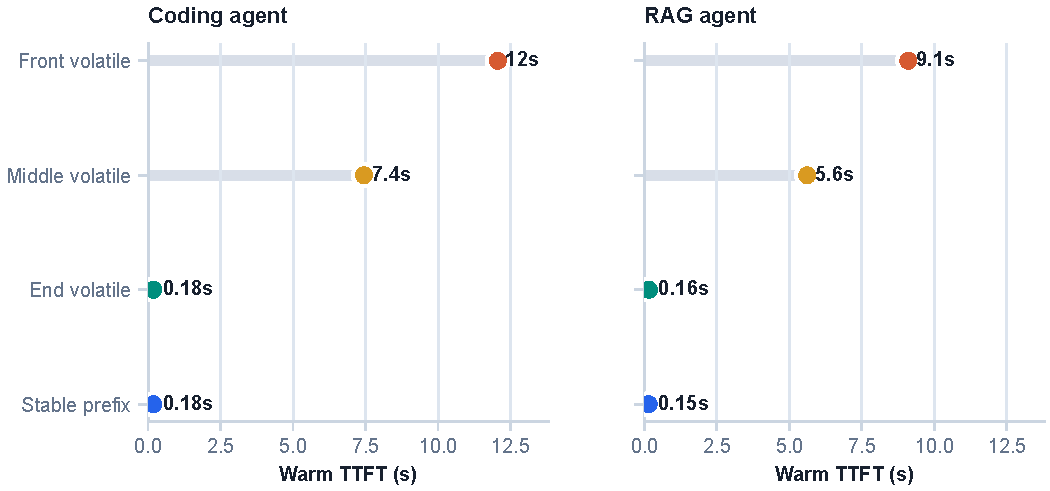
\includegraphics[width=\linewidth]{report_layout_sensitivity_8k}
    \caption{8K prompt 下动态字段位置对 warm TTFT 的影响。}
    \label{fig:layout}
  \end{minipage}\hfill
  \begin{minipage}[t]{0.49\linewidth}
    \vspace{0pt}
    \captionof{table}{\textbf{8K 布局敏感性实验结果。}}
    \label{tab:layout}
    \centering
    \scriptsize
    \setlength{\tabcolsep}{1pt}
    \begin{tabular*}{\linewidth}{@{\extracolsep{\fill}}ll
      S[table-format=2.3,detect-weight=true]
      S[table-format=2.1,detect-weight=true]@{}}
      \toprule
      \textbf{负载} & \textbf{布局}
        & {\makecell[c]{\textbf{中位 TTFT}\textbf{(s)}}}
        & {\makecell[c]{\textbf{相对 front-volatile}\textbf{加速 ($\times$)}}} \\
      \midrule
      \multirow{4}{*}{Coding}
        & \texttt{front\_volatile}  & 12.062 & 1.0 \\
        & \texttt{middle\_volatile} & 7.446  & 1.6 \\
        & \texttt{end\_volatile}    & \bfseries 0.179  & \bfseries 67.3 \\
        & \texttt{stable\_prefix}   & 0.180  & 67.2 \\
      \midrule
      \multirow{4}{*}{RAG}
        & \texttt{front\_volatile}  & 9.104  & 1.0 \\
        & \texttt{middle\_volatile} & 5.616  & 1.6 \\
        & \texttt{end\_volatile}    & 0.161  & 56.4 \\
        & \texttt{stable\_prefix}   & \bfseries 0.153  & \bfseries 59.4 \\
      \bottomrule
    \end{tabular*}
  \end{minipage}
\end{figure}

布局敏感性实验解释了主实验中 S1 为什么失效。所有组都打开 \texttt{--cache-prompt}，但 \texttt{front\_volatile} 会让每轮请求从第一个 token 开始就发生变化，服务端无法复用长前缀；\texttt{middle\_volatile} 只能复用动态字段之前的一段内容，因此收益有限。8K Coding 中，\texttt{middle\_volatile} 的 TTFT 为 7.446 秒，只比 \texttt{front\_volatile} 快 1.6$\times$；RAG 中也只有 1.6$\times$。这与构造方式相符：动态字段被插入稳定上下文中部后，前半段可以命中，后半段仍需重新 prefill，因此它不会接近完整稳定前缀的表现。

\texttt{end\_volatile} 和 \texttt{stable\_prefix} 的结果几乎重合，说明关键变量不是动态字段是否存在，而是它是否切断稳定前缀。8K Coding 中，两者分别为 0.179 秒和 0.180 秒；8K RAG 中，两者分别为 0.161 秒和 0.153 秒。相对于 \texttt{front\_volatile}，这对应 56$\times$--67$\times$ 的加速。换到真实 Agent 系统中，这意味着系统指令、工具 schema、仓库摘要、检索文档和长期记忆摘要应形成一个字节级稳定的头部区域；当前时间、trace id、turn id、最新错误日志、工具返回和当前用户请求则应集中后置。否则，即使后面 90\% 的内容没有语义变化，也会因为前缀 token 序列不一致而被迫重新计算。

这个实验也提示了一个容易被忽视的工程风险：许多 Agent 框架会在 prompt 开头插入“当前时间”“会话 id”“已用 token 数”或随机顺序的 JSON 字段，这些字段对模型语义帮助有限，却会破坏后续全部稳定内容的复用。相比之下，把这些字段移动到用户消息或末尾状态块中，不改变任务信息量，却能把 warm TTFT 从秒级降到百毫秒级。因此，prompt 布局不是文案整理问题，而是推理服务接口的一部分。

\subsection{\texorpdfstring{\texttt{--cache-reuse} 参数扫描}{--cache-reuse 参数扫描}}
\label{sec:cache-reuse}

\begin{figure}[H]
  \centering
  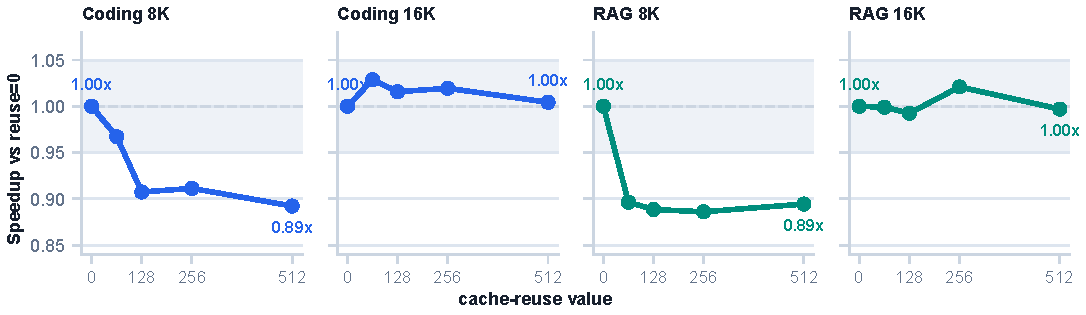
\includegraphics[width=\linewidth]{report_cache_reuse_sweep}
  \caption{\texttt{--cache-reuse} 参数扫描。}
  \label{fig:cache-reuse}
\end{figure}

图~\ref{fig:cache-reuse} 以 \texttt{reuse=0} 为基准显示 TTFT 加速比，灰色带对应 $\pm$5\% 区间。参数扫描结果表明，在稳定前缀已经提供主要收益之后，继续调节 \texttt{--cache-reuse} 的边际影响较小。8K Coding 负载中，reuse=64、128、256、512 的 TTFT 均慢于 reuse=0，其中 reuse=512 约慢 10.8\%；8K RAG 也类似，非零 reuse 大约慢 10\%--11\%。到 16K 时，差异进一步收窄：Coding 的最佳点是 reuse=64，比 reuse=0 快约 2.9\%；RAG 的最佳点是 reuse=256，比 reuse=0 快约 2.1\%。

这组结果说明，\texttt{--cache-reuse} 更像是对已经存在的缓存匹配和 KV shifting 行为做细节调节，而不是一个能独立产生大幅加速的开关。在本文的单会话、单并发、稳定前缀设置下，连续请求天然共享同一个长前缀，主要收益已经由 prompt 布局获得；reuse 参数只能影响剩余边界处理和小块复用策略。与此相比，布局实验中把动态字段从前部移动到末尾可以带来 50$\times$ 以上差距。因此，实际调优顺序应当是先保证稳定前缀，再根据多会话、上下文接近上限或 slot 频繁切换等更复杂场景考虑 reuse 参数。

\subsection{内存占用与吞吐}
\label{sec:memory-throughput}

\begin{figure}[H]
  \centering
  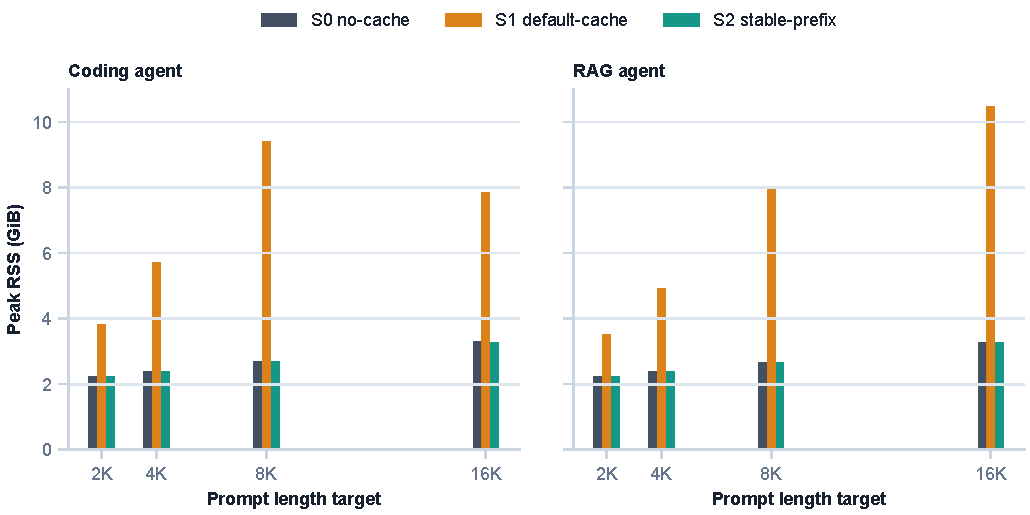
\includegraphics[width=\linewidth]{report_memory_by_strategy}
  \caption{不同策略的服务端峰值 RSS。}
  \label{fig:memory}
\end{figure}

内存结果表明，在 2K--16K 范围内，3B Q4 模型适合当前 32 GB unified memory 机器。S2 的峰值 RSS 从约 2.28 GiB 增至约 3.36 GiB；S0 也处在相近水平，说明稳定前缀缓存并没有在本实验范围内引入不可接受的额外常驻内存。更值得注意的是 S1：8K Coding 负载达到 9622.7 MiB，16K RAG 负载达到 10719.0 MiB，明显高于 S0/S2。它的性能却没有改善，说明缓存状态本身会占用内存；如果 prompt 组织方式导致命中失败，这部分内存开销就不会转化为 TTFT 收益。

RSS 不应被解读为严格的逐 token KV cache 公式。它还包含模型权重、Metal 后端缓冲区、server 运行时分配和缓存管理状态，因此不同策略之间可能出现非单调波动。对本文问题而言，更重要的是性价比：S2 在保持 3.4 GiB 左右峰值 RSS 的同时获得百倍级 TTFT 加速；S1 消耗更多内存却接近 S0 的延迟。这进一步支持本文的主张：本地 Agent 首先要约束 prompt 结构，否则单纯启用缓存既可能无效，也可能增加资源占用。

吞吐结果也需要结合输出长度解释。S2 并没有显著改变模型逐 token decode 的能力，Coding 负载在 16K S2 下的 decode 吞吐下降到约 33 token/s，RAG 仍约 43 token/s；这些变化更可能来自输出长度、采样结束位置和运行时抖动，而不是 prompt cache 直接加速 decode。prompt cache 的主要价值在于去掉首 token 之前的大段重复 prefill，使交互从“等待完整长上下文处理完”转变为“快速进入正常 decode”。因此，TTFT 是本实验最敏感、也最能反映 Agent 交互体验的指标。

\section{结论}
\label{sec:conclusion}

在本机 llama.cpp + Qwen2.5-Coder-3B 的实验条件下，prompt/KV 缓存可以把长上下文本地 Agent 的 warm TTFT 从秒级到几十秒级降到百毫秒级，但前提是 prompt 具有长且稳定的可复用前缀。仅打开缓存不足以获得收益；如果动态字段位于 prompt 前部，性能几乎等同于关闭缓存，并且可能增加 RSS。

因此，对本地 coding agent 和 RAG agent 来说，更有效的优化顺序是先建立稳定前缀协议，再考虑 \texttt{--cache-reuse}、并发 slot、上下文长度和模型量化等细节参数。系统指令、工具定义、仓库摘要、固定文档上下文和长期记忆摘要等稳定内容应放在 prompt 前部，并保持跨轮字节级稳定；时间戳、request id、turn id、当前错误日志、工具返回和当前用户请求等动态内容则应集中后置。Agent 框架也应把 prompt 组装视为性能敏感路径，避免在稳定前缀中插入随机顺序的 JSON 字段、当前时间、临时路径、计数器或日志片段。

不过，本文仍存在若干限制。为了隔离变量，实验负载采用合成方式构造，因此无法覆盖真实大型代码库、真实检索系统以及多用户交替会话中的全部复杂性。实验仅在单并发条件下进行，尚未测量多 slot 并发场景中缓存可能发生的抢占或污染。模型方面，本文固定使用 Qwen2.5-Coder-3B Q4\_K\_M，因此绝对延迟结果不能直接外推到 7B、14B 模型或其他推理后端。尽管如此，布局实验只改变动态字段的位置，变量控制较为明确，因而具有较强的因果解释力，“稳定前缀优先”的判断应当能够迁移到多数支持 prompt 缓存的实现中。

\end{document}
